This is another important layer in our design. This part of the system works as a bridge between the User Interface and the Database of the system. If the data is being received from the UI controller that are coming form different subsections of UI, the Business controller will, depending upon what kind of input it gets, either generate an AR, generate a Qr or does an input validation. The Business Logic will send the data to the data base for more validation and verification or to store the data in database. If Business Logic is getting the instruction to fetch data form Database, then it will contact Database to get particular data, which is then passed on to the UI.

\subsection{Layer Hardware}
A description of any involved hardware components for the layer. For example, if each subsystem is a software process running on an embedded computer, discuss the specifics of that device here. Do not list a hardware component that only exists at the subsystem level (include it in the following sections).

\subsection{Layer Operating System}
iOS/Android

\subsection{Layer Software Dependencies}
This layer is build using ReactNative. Dependencies we needed for this part are
\begin{rand}"dependencies":\\ {
    "expo": "34.0.1",\\
    "expo-barcode-scanner": "6.0.0",\\
    "expo-permissions": "6.0.0",\\
    "firebase": "6.6.0",\\
    "native-base": "2.13.7",\\
    "react": "16.8.3",\\
    "react-dom": "16.8.6",\\
    "react-native": "https://github.com/expo/react-native/archive/sdk-34.0.0.tar.gz",\\
    "react-native-datepicker": "1.7.2",\\
    "react-native-gesture-handler": "1.4.1",\\
    "react-native-search-bar": "3.4.3",\\
    "react-native-simple-radio-button": "2.7.3",\\
    "react-native-vector-icons": "6.6.0",\\
    "react-native-web": "0.11.4",\\
    "react-navigation": "4.0.0",\\
    "react-navigation-stack": "1.5.1",\\
    "reinput": "3.7.1"]\\
\end{rand}
\subsection{Business Controller}
Any kind of data coming and going to Business Logic do so through the Business controller. The data coming to Business Logic will be divided into three different ways, namely AR generation, QR generation or Input Validation related. Depending upon those different input types, Business controller communicates with the Database controller to get particular data or to store that information.

\begin{figure}[h!]
	\centering
 	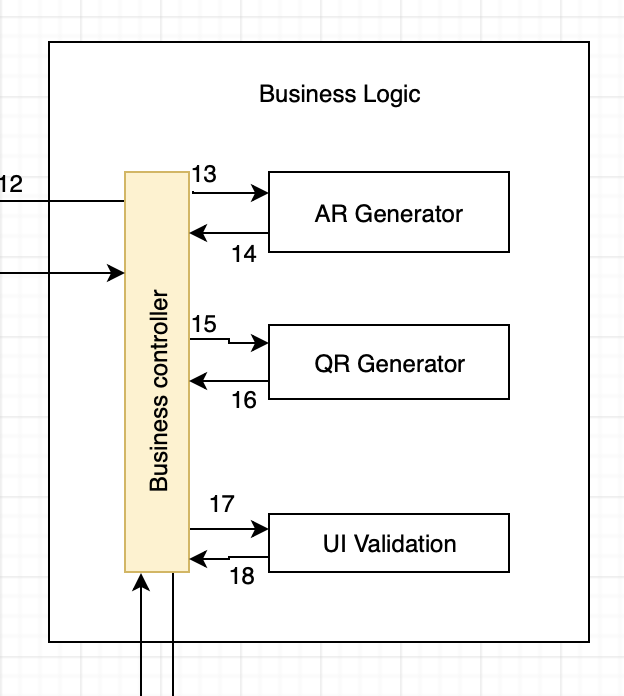
\includegraphics[width=0.60\textwidth]{images/businesscontroller}
 \caption{Example subsystem description diagram}
\end{figure}

\subsubsection{Subsystem Hardware}
NA

\subsubsection{Business Controller Operating system}
iOS/Andriod

\subsubsection{Business Controller Software Dependencies}
A description of any software dependencies (libraries, frameworks, design software for mechanical parts or circuits, etc) required by the subsystem.

\subsubsection{Business Controller Programming Languages}
JavaScript

\subsubsection{Subsystem Data Structures}
JSON, Array, Union, List.

\subsubsection{Business Controller Data Processing}
Shorting Algorithm was used.

\subsection{AR Generator}
AR generator is the part of Business logic that generates AR when a customer wants to store an item to the shelf. The generated AR is then used when the customer wants to search the item. When the customer wants to search an item, he will scan bar-code or enter manually. Then the program will display the AR right on the bar-code of the item.
\begin{figure}[h!]
	\centering
 	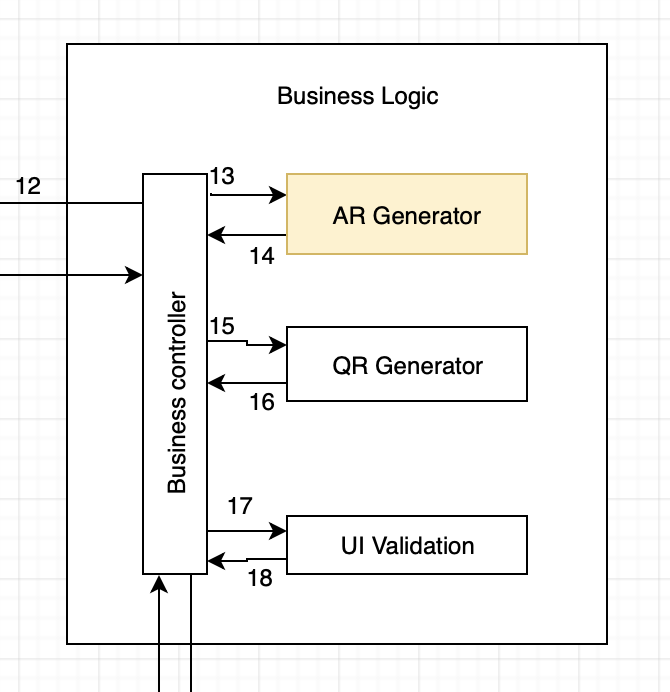
\includegraphics[width=0.60\textwidth]{images/argenerator}
 \caption{AR Generator}
\end{figure}

\subsubsection{AR Generator Hardware}
Phone Camera

\subsubsection{AR Generator Operating System}
iOS/Andriod

\subsubsection{AR Generator Software Dependencies}
Phone camera, images available

\subsubsection{AR Generator Programming Languages}
JavaScript

\subsubsection{AR Generator Data Structures}
JSON, Array, Union, List.

\subsubsection{AR Generator Data Processing}
Shorting Algorithm was used.


\subsection{QR Generator}
Based on description of the item customer provides, QR generator generate QR.This QR is then store in the database along with the  description of the item.

\begin{figure}[h!]
	\centering
 	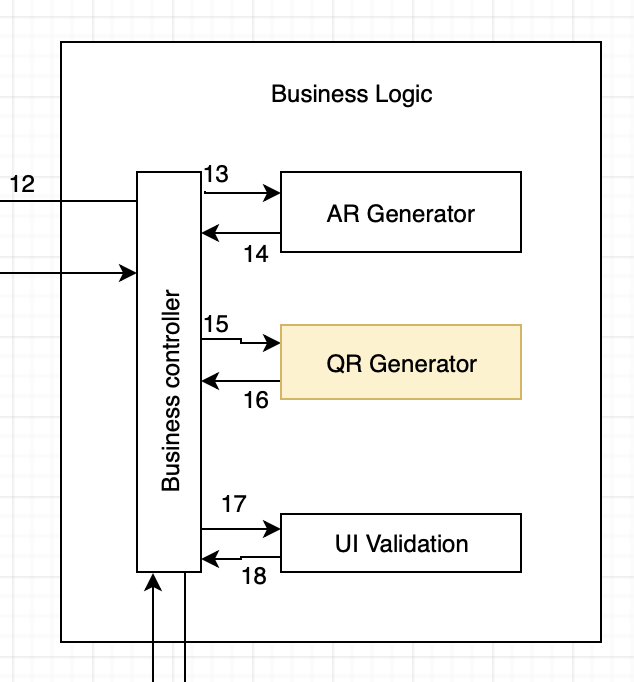
\includegraphics[width=0.60\textwidth]{images/qrgenerator}
 \caption{QR Generator}
\end{figure}

\subsubsection{QR Generator Hardware}
Phone Camera

\subsubsection{QR Generator Operating System}
iOS/Andriod

\subsubsection{QR Generator Software Dependencies}
Phone camera

\subsubsection{QR Generator Programming Languages}
JavaScript

\subsubsection{QR Generator Data Structures}
JSON, Array, Union, List.



\subsection{UI Input Validation}
This section will validate format and types of input from users. It will reject the inputs if user's input is wrong format and suggest the correct format of the input.Provide guidance on how to fix any errors, don't just tell users what they did wrong. It will prevent from unauthorized SQL injection into the data base.

\begin{figure}[h!]
	\centering
 	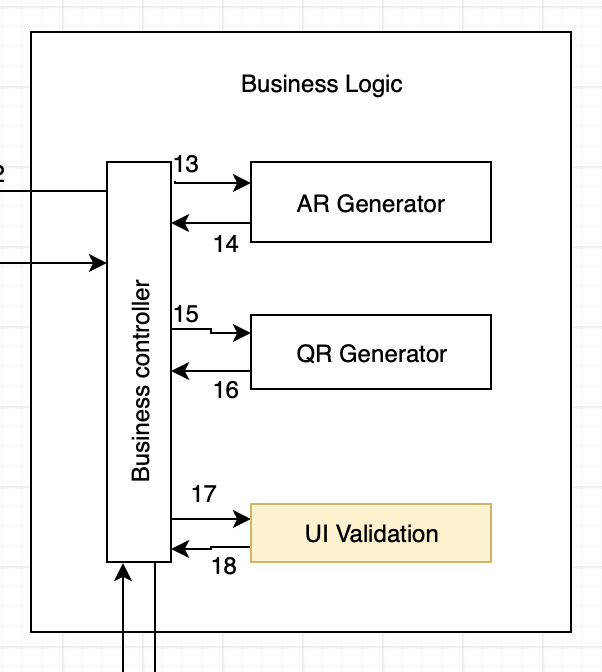
\includegraphics[width=0.60\textwidth]{images/uivalidation}
 \caption{UI Validation}
\end{figure}

\subsubsection{Input Validation Hardware}
N/A

\subsubsection{Input Validation Operating System}
iOS/Android

\subsubsection{Input Validation Software Dependencies}


\begin{rand}"dependencies":\\ {
    "expo": "34.0.1",\\
    "expo-barcode-scanner": "6.0.0",\\
    "expo-permissions": "6.0.0",\\
    "react": "16.8.3",\\
    "react-native": "https://github.com/expo/react-native/archive/sdk-34.0.0.tar.gz",\\
    "react-native-datepicker": "1.7.2",\\
    "react-native-simple-radio-button": "2.7.3",\\
    "react-native-vector-icons": "6.6.0",\\
    "react-navigation-stack": "1.5.1",\\
    "reinput": "3.7.1"]\\
\end{rand}

\subsubsection{Input Validation Programming Languages}
JavaScript

\subsubsection{Input Validation Data Structures}
JSON, Array, Union, List.
